\documentclass[fleqn]{jbook}
\usepackage{physpub}
\begin{document}
\begin{question}{問題9}{田中雄、芝隼人}
幅$b$を持つ矩形ポテンシャル障壁$V(z)$による一次元電子の散乱を考える。$V(z)$の左$(z=-\infty )$から入射する電子の波動関数を$\psi_l$、右から入射する電子のそれを$\psi_r$とすると、図1の様に$z<-b/2$及び$z>b/2$で
\begin{eqnarray}
\psi_l (z)=\left\{ 
\begin{array}{ll}{}
\exp [ikz]+R\exp [-ikz] & z<-b/2 \\
T \exp [ikz] & z>b/2 
\end{array}
\right.
\end{eqnarray}
及び
\begin{eqnarray}
\psi_r (z) = \left\{ 
\begin{array}{ll}{}
T\exp [-ikz] & z< -b/2 \\
\exp [-ikz] +R \exp [ikz] & z> b/2 
\end{array}
\right.
\end{eqnarray}
と表される。ただし、$T,R$はそれぞれ透過係数及び反射係数であり、$T= e^{i\alpha}\sin (\gamma ),\ R= ie^{i\alpha}\cos (\gamma )$の様に位相差$\alpha$と散乱振幅に関係した量$\gamma$で表される。また、波数$k$は電子のエネルギー$E$と質量$m$を用いて次のように書ける。
\begin{eqnarray}
k=\sqrt{2mE}/\hbar
\end{eqnarray}
\begin{enumerate}
\item
波動関数の一般解$\psi$は
\begin{eqnarray}
\psi (z) =\left\{
\begin{array}{ll}{}
A_{-1}\exp [ikz] +B_{-1}\exp [-ikz] & z< -b/2 \\
A_0 \exp [ikz] + B_0 \exp [-ikz] & z> b/2 
\end{array}
\right. \end{eqnarray}
の様に書ける(図2)。一般解が線形独立解$\psi_r , \psi_l$の重ね合わせで書ける事を利用して、$A_{-1},B_{-1}$と$A_0, B_0$の関係式を導け。また、それを式(5)の様に行列表示した時の、行列要素を$\alpha , \gamma$で表せ。($M$は転送行列と呼ばれる。)
\begin{eqnarray}
\left( \begin{array}{c}{}
A_0 \\ B_0 
\end{array}\right) =M \left(
\begin{array}{c}{}
A_{-1} \\ B_{-1} 
\end{array}\right) 
\end{eqnarray}
\end{enumerate}

\begin{figure}[h]
  \begin{center}
    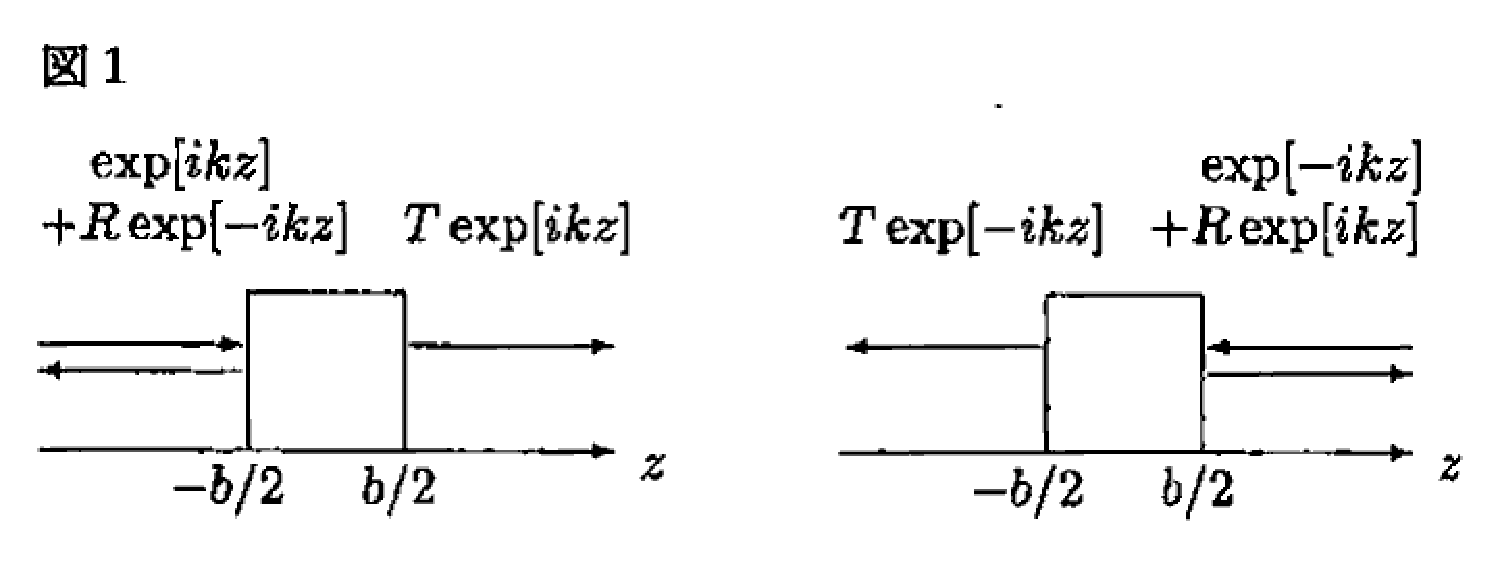
\includegraphics[width=110mm]{2003phy9-1.eps}
  \end{center}
\end{figure}

\begin{figure}[h]
  \begin{center}
    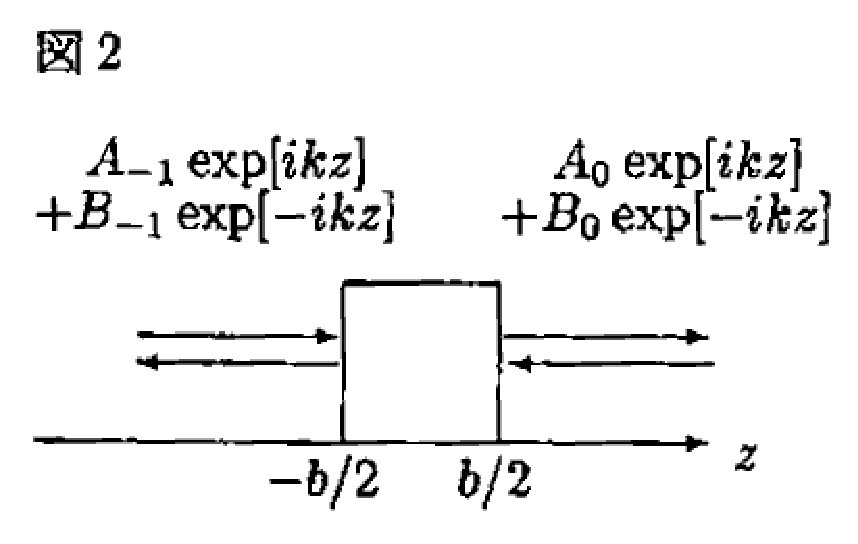
\includegraphics[width=58mm]{2003phy9-2.eps}
  \end{center}
\end{figure}

\begin{figure}[h]
  \begin{center}
    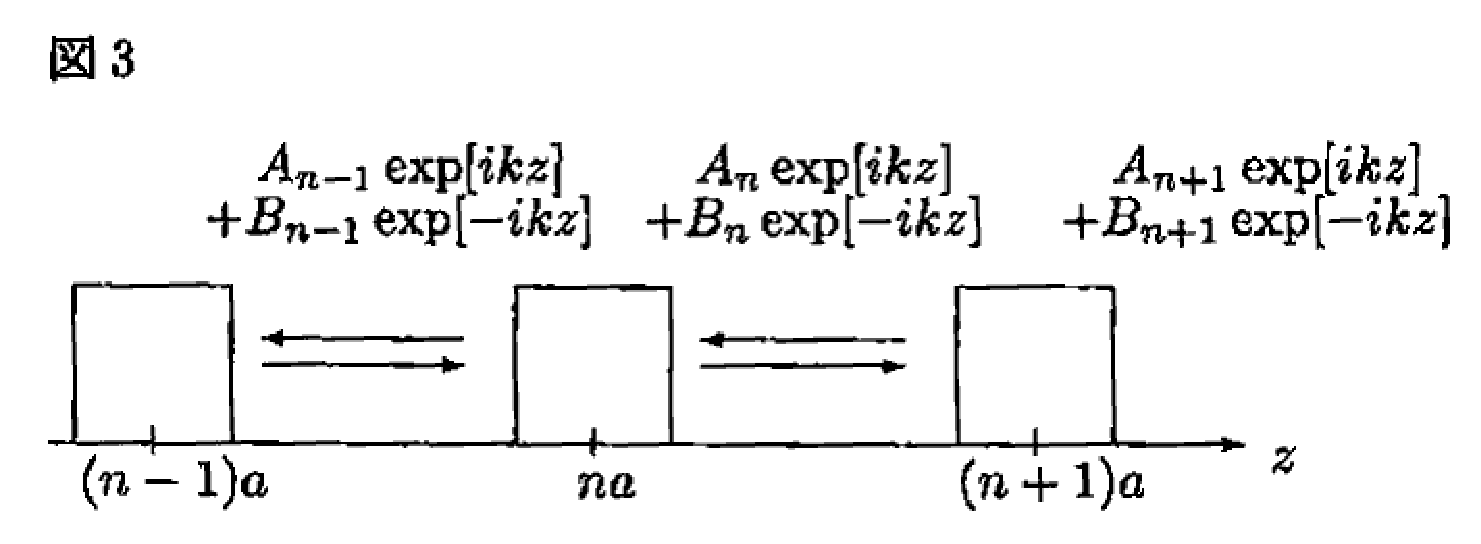
\includegraphics[width=110mm]{2003phy9-3.eps}
  \end{center}
\end{figure}

次に$V(z)$が間隔$a (>b)$で等間隔に並んでいる時(すなわち一次元周期系)の電子状態を考える。図3のように波動関数$\Psi$は$na<z< (n+1)a$かつポテンシャルがゼロになる領域で$A_n \exp [ikz] +B_n \exp [-ikz]$と書ける。今、$-a+b/2 < z< a-b/2$に注目し、$\Psi$がこの領域で線形独立解$\psi_r,\psi_l$の重ね合わせで書ける事を利用すると、ここでも式(5)が成り立つ事、また一般に以下の関係が成り立つ事がわかる。
\begin{eqnarray}
\left( \begin{array}{c}{}
A_n \\ B_n 
\end{array}\right) =M \left(
\begin{array}{c}{}
A_{n-1} \\ B_{n-1}
\end{array} \right) 
\end{eqnarray}

\begin{enumerate}\setcounter{enumi}{1}
\item
周期系の波動関数$\Psi$はブロッホ条件$\Psi (z+a) = \exp [iqa] \Psi (z)$を満たす事が知られている。この条件を用いて$A_n, B_n$が満たすべき関係式を示せ。ただし、$q$はブロッホ波数である。(波数$k$は式(3)によって定義されるエネルギーの関数であり、ブロッホ波数$q$とは直接関係するものではない事に留意せよ。)
\item
ブロッホ条件と式(6)が同時に成り立つ時、$q$と$k$は次の式で関係付けられる事を示せ。
\begin{eqnarray}
\cos (qa) = \frac{ \cos (ka+\alpha )}{\sin (\gamma )}
\end{eqnarray}
\end{enumerate}
次に、$\alpha ,\gamma$が波数$k$を介して
\begin{eqnarray}
\gamma =\frac{\pi}{2} \frac{k}{k_c},\quad \alpha = -c\frac{k}{k_c}
\end{eqnarray}
の様にエネルギーに依存している場合を考える。ただし、$k_c, c$は定数であり、$\pi/2 <k_c a-c$を満たす。以下、$0<k<k_c$で示されるエネルギー範囲で考えよ。
\begin{enumerate}\setcounter{enumi}{3}
\item
式(7)の右辺の値を波数$k$の関数としてプロットせよ。
\item
$ka +\alpha$が$\pi$の整数倍の時、式(7)を満たす実数の$q$が存在しない事を示し、その物理的意味を述べよ。
\item 
実数の$q$が存在するための$k$の条件を$k_c,c,a$を用いて示せ。
\item 
$k_c a-c=5\pi /2$の場合、$q$と$E$の関係式(すなわち分散関係)の概略図を示せ。


\end{enumerate}
\end{question}
\begin{answer}{問題9}{田中雄、芝隼人}
\begin{enumerate}
\item
一般解が$\psi_l ,\psi_r $の波動関数の重ね合わせとして、
\[
\psi =a\psi_l +b\psi_r
\]
として得られるとおく。(1),(2)式を上式に代入して(4)を比較することにより次の式が得られる。
\begin{eqnarray}
\left\{
\begin{array}{rl}{}
A_{-1}\exp [ikz]+B_{-1}\exp [-ikz] =& a\exp [ikz]+aR\exp [-ikz]+bT\exp [-ikz]  \\
A_{0}\exp [ikz]+B_{0}\exp [-ikz] =& aT\exp [ikz]+b\exp [-ikz]+bR\exp [ikz]
\end{array}
\right.
\end{eqnarray}
従って、
\begin{eqnarray}
A_{-1} = a,\quad B_{-1} =aR +bT \\
A_0 =aT +bR,\quad B_0 = b
\end{eqnarray}
$a,b$を消去することにより関係式
\begin{eqnarray}
\left\{ \begin{array}{l}{}
A_0 = \displaystyle TA_{-1} + (B_{-1} -RA_{-1} )\frac{R}{T} \\
B_0 = \displaystyle(B_{-1} -RA_{-1} )\frac{1}{T}
\end{array}\right.
\end{eqnarray}
が立つ。転送行列$M$を構成すると、
\begin{eqnarray}
M= \left( \begin{array}{cc}{}
T-\displaystyle\frac{R^2}{T} & \displaystyle\frac{R}{T} \\ 
-\displaystyle\frac{R}{T} & \displaystyle\frac{1}{T}
\end{array}\right) = \left( \begin{array}{cc}{}
\displaystyle\frac{e^{i\alpha}}{\sin (\gamma) } & i \cot (\gamma ) \\
-i\cot (\gamma ) & \displaystyle\frac{e^{-i\alpha}}{\sin (\gamma ) }
\end{array} \right)
\end{eqnarray} 

\item
周期系の波動関数であることより
\begin{equation}
\Phi (z+a)=A_{n+1}e^{\imath ka}e^{\imath kz}+B_{n+1}e^{-\imath ka}e^{-\imath kz}
\end{equation}
である。また、Bloch条件より
\begin{equation}
\Phi (z+a)=e^{\imath qa}\Phi (z) = A_{n}e^{\imath qa}e^{\imath kz}+B_{n}e^{\imath qa}e^{-\imath kz}
\end{equation}
(14),(15)より求める関係式は、
\begin{equation}
\left\{
  \begin{array}{c}
    A_{n+1}=A_{n}e^{\imath (q-k)a}   \\
    B_{n+1}=B_{n}e^{\imath (q+k)a}   \\
  \end{array}
\right.
\end{equation}
となる。\\

\item
1,2の結果と問題文中の(6)を用いると、
\begin{eqnarray}
\left(
  \begin{array}{c}
    A_{n+1}   \\
    B_{n+1}   \\
  \end{array}
\right)
&=&M
\left(
  \begin{array}{c}
    A_{n}   \\
    B_{n}   \\
  \end{array}
\right)\\
&=&
\left(
  \begin{array}{cc}
    e^{\imath \alpha }\textrm{cosec} (\gamma )   & \imath \cot (\gamma )   \\
    -\imath \cot (\gamma )   & e^{-\imath \alpha }\textrm{cosec} (\gamma )   \\
  \end{array}
\right)
\left(
  \begin{array}{c}
    A_{n}   \\
    B_{n}   \\
  \end{array}
\right)
\end{eqnarray}
となる。これを解くと、
\begin{eqnarray}
&& \left(
  \begin{array}{c}
    A_{n}e^{\imath (q-k)a}   \\
    B_{n}e^{\imath (q+k)a}   \\
  \end{array}
\right)\sin(\gamma)
=
\left(
  \begin{array}{c}
    A_{n}e^{\imath \alpha}+\imath B_{n}\cos (\gamma)    \\
    -\imath A_{n}\cos (\gamma)+B_{n}e^{-\imath \alpha}  \\
  \end{array}
\right)\\
&& \Leftrightarrow  \left\{
  \begin{array}{c}
    A_{n}(e^{\imath (q-k)a}\sin (\gamma)-e^{\imath \alpha})=\imath B_{n}\cos (\gamma)   \\
    B_{n}(e^{\imath (q+k)a}\sin (\gamma)-e^{-\imath \alpha})=-\imath A_{n}\cos (\gamma)   \\
  \end{array}
\right.
\end{eqnarray}
2式を用いて、$A_{n},B_{n}$を消去すると、
\begin{eqnarray}
\cos (qa)=\frac{\cos (ka+\alpha )}{\sin (\gamma)}
\end{eqnarray}
となる。\\

\item
\begin{equation}
ka+\alpha = \frac{k}{k_{c}}(k_{c}a-c) > \frac{\pi}{2}\frac{k}{k_{c}} = \gamma
\end{equation}
であることから、グラフは$0<k<k_{c}$の範囲では以下のようになる。(図は$k_ca-c=6\pi$の場合を示した。)
\begin{center}
\input{2003phy9-4.tpc}
\end{center}
\item
$ka+\alpha=n\pi \ $($n$は整数)のとき、$|\cos (ka+\alpha )|=1$であり、また$\gamma =\frac{\pi}{2}\frac{k}{k_{c}}\ (0<k<k_{c})$のとき$\sin (\gamma)<1$であるので、
\begin{equation}
\left|\frac{\cos (ka+\alpha )}{\sin (\gamma)}\right|>1
\end{equation}
となる。従って題意のような$q$は存在しない。

この条件は上図のグラフが$\pm 1$の直線ではさまれた領域の中にないことを意味している。従って、$\cos (qa)=\frac{\cos (ka+\alpha )}{\cos (\gamma)}$を満たす実数$q$は存在せずBloch条件を満たせないので、そのような周期系の波動関数は存在しないことが分かる。したがって、$ka+\alpha=n\pi $で計算されるエネルギーの準位が禁止される。\\

\item
$|\cos (qa)|\le 1$、つまり$\displaystyle\left|\frac{\cos (\frac{k}{k_{c}}(k_{c}a-c))}{\sin (\frac{\pi}{2}\frac{k}{k_{c}})}\right|=\left|\frac{\cos (\frac{k}{k_{c}}(k_{c}a-c))}{\cos (\frac{\pi}{2}-\frac{\pi}{2}\frac{k}{k_{c}})}\right|\le 1$であればよい。このとき、
\begin{equation}
-\frac{\pi}{2}\frac{k}{k_{c}}+\frac{\pi}{2}(2n+1) \le \frac{k}{k_{c}}(k_{c}a-c) \le \frac{\pi}{2}\frac{k}{k_{c}}+\frac{\pi}{2}(2n+1) \ \ (nは整数)
\end{equation}
であるので、$k$について解くと、
\begin{equation}
\displaystyle\frac{n+\frac{1}{2}}{\frac{k_{c}a-c}{\pi}+ \frac{1}{2}}\le \frac{k}{k_{c}} \le \frac{n+\frac{1}{2}}{\frac{k_{c}a-c}{\pi}-\frac{1}{2}}
\end{equation}
という条件を得る。ただし、$0<k<k_{c}$であるので、$n=0,1,2,,...$であり、さらに場合分けすると、
\begin{eqnarray}
\left \{
  \begin{array}{ll}{}
\displaystyle    \frac{n+\frac{1}{2}}{\frac{k_{c}a-c}{\pi}+ \frac{1}{2}}\le \frac{k}{k_{c}} \le \frac{n+\frac{1}{2}}{\frac{k_{c}a-c}{\pi}-\frac{1}{2}} & \displaystyle \left(n\le \frac{k_{c}a-c}{\pi}-1 \right)  \\
\displaystyle    \frac{n+\frac{1}{2}}{\frac{k_{c}a-c}{\pi}+ \frac{1}{2}}\le \frac{k}{k_{c}} \le 1 & \displaystyle\left(\frac{k_{c}a-c}{\pi}-1 < n\le \frac{k_{c}a-c}{\pi}\right) \\
    &\qquad\qquad (ただし、n =0,1,2, \ldots)\\
  \end{array}
\right.
\end{eqnarray}
を得る。以上の範囲以外のの$n$が存在しないことは(25)式から分かる。\\

\item
6.での結果に$k_{c}a-c=\frac{5\pi}{2}$を代入すると、
\begin{equation}
\frac{k_{c}}{3}(n+\frac{1}{2}) \le k \le \frac{k_{c}}{2}(n+\frac{1}{2})
\end{equation}
となる。さらに$0<k<k_{c}$を満たすような$n$を選ぶと許されるのは結局、
\begin{equation}
\frac{1}{6}k_{c} \le k \le \frac{1}{4}k_{c}, \ \ 
\frac{1}{2}k_{c} \le k \le \frac{3}{4}k_{c}, \ \
\frac{5}{6}k_{c} \le k < k_{c}
\end{equation}
のみ。さらに、$E_{0}\equiv \frac{\hbar k_{c}^{2}}{2m}$とすれば、エネルギー$E$について、
\begin{equation}
\frac{1}{36}E_{0} \le E \le \frac{1}{16}E_{0}, \ \ 
\frac{1}{4}E_{0} \le E \le \frac{9}{16}E_{0}, \ \
\frac{25}{36}E_{0} \le E < E_{0}
\end{equation}
となる。従って分散関係の概略は以下のようになる。

\begin{figure}[htbp]
  \begin{center}
    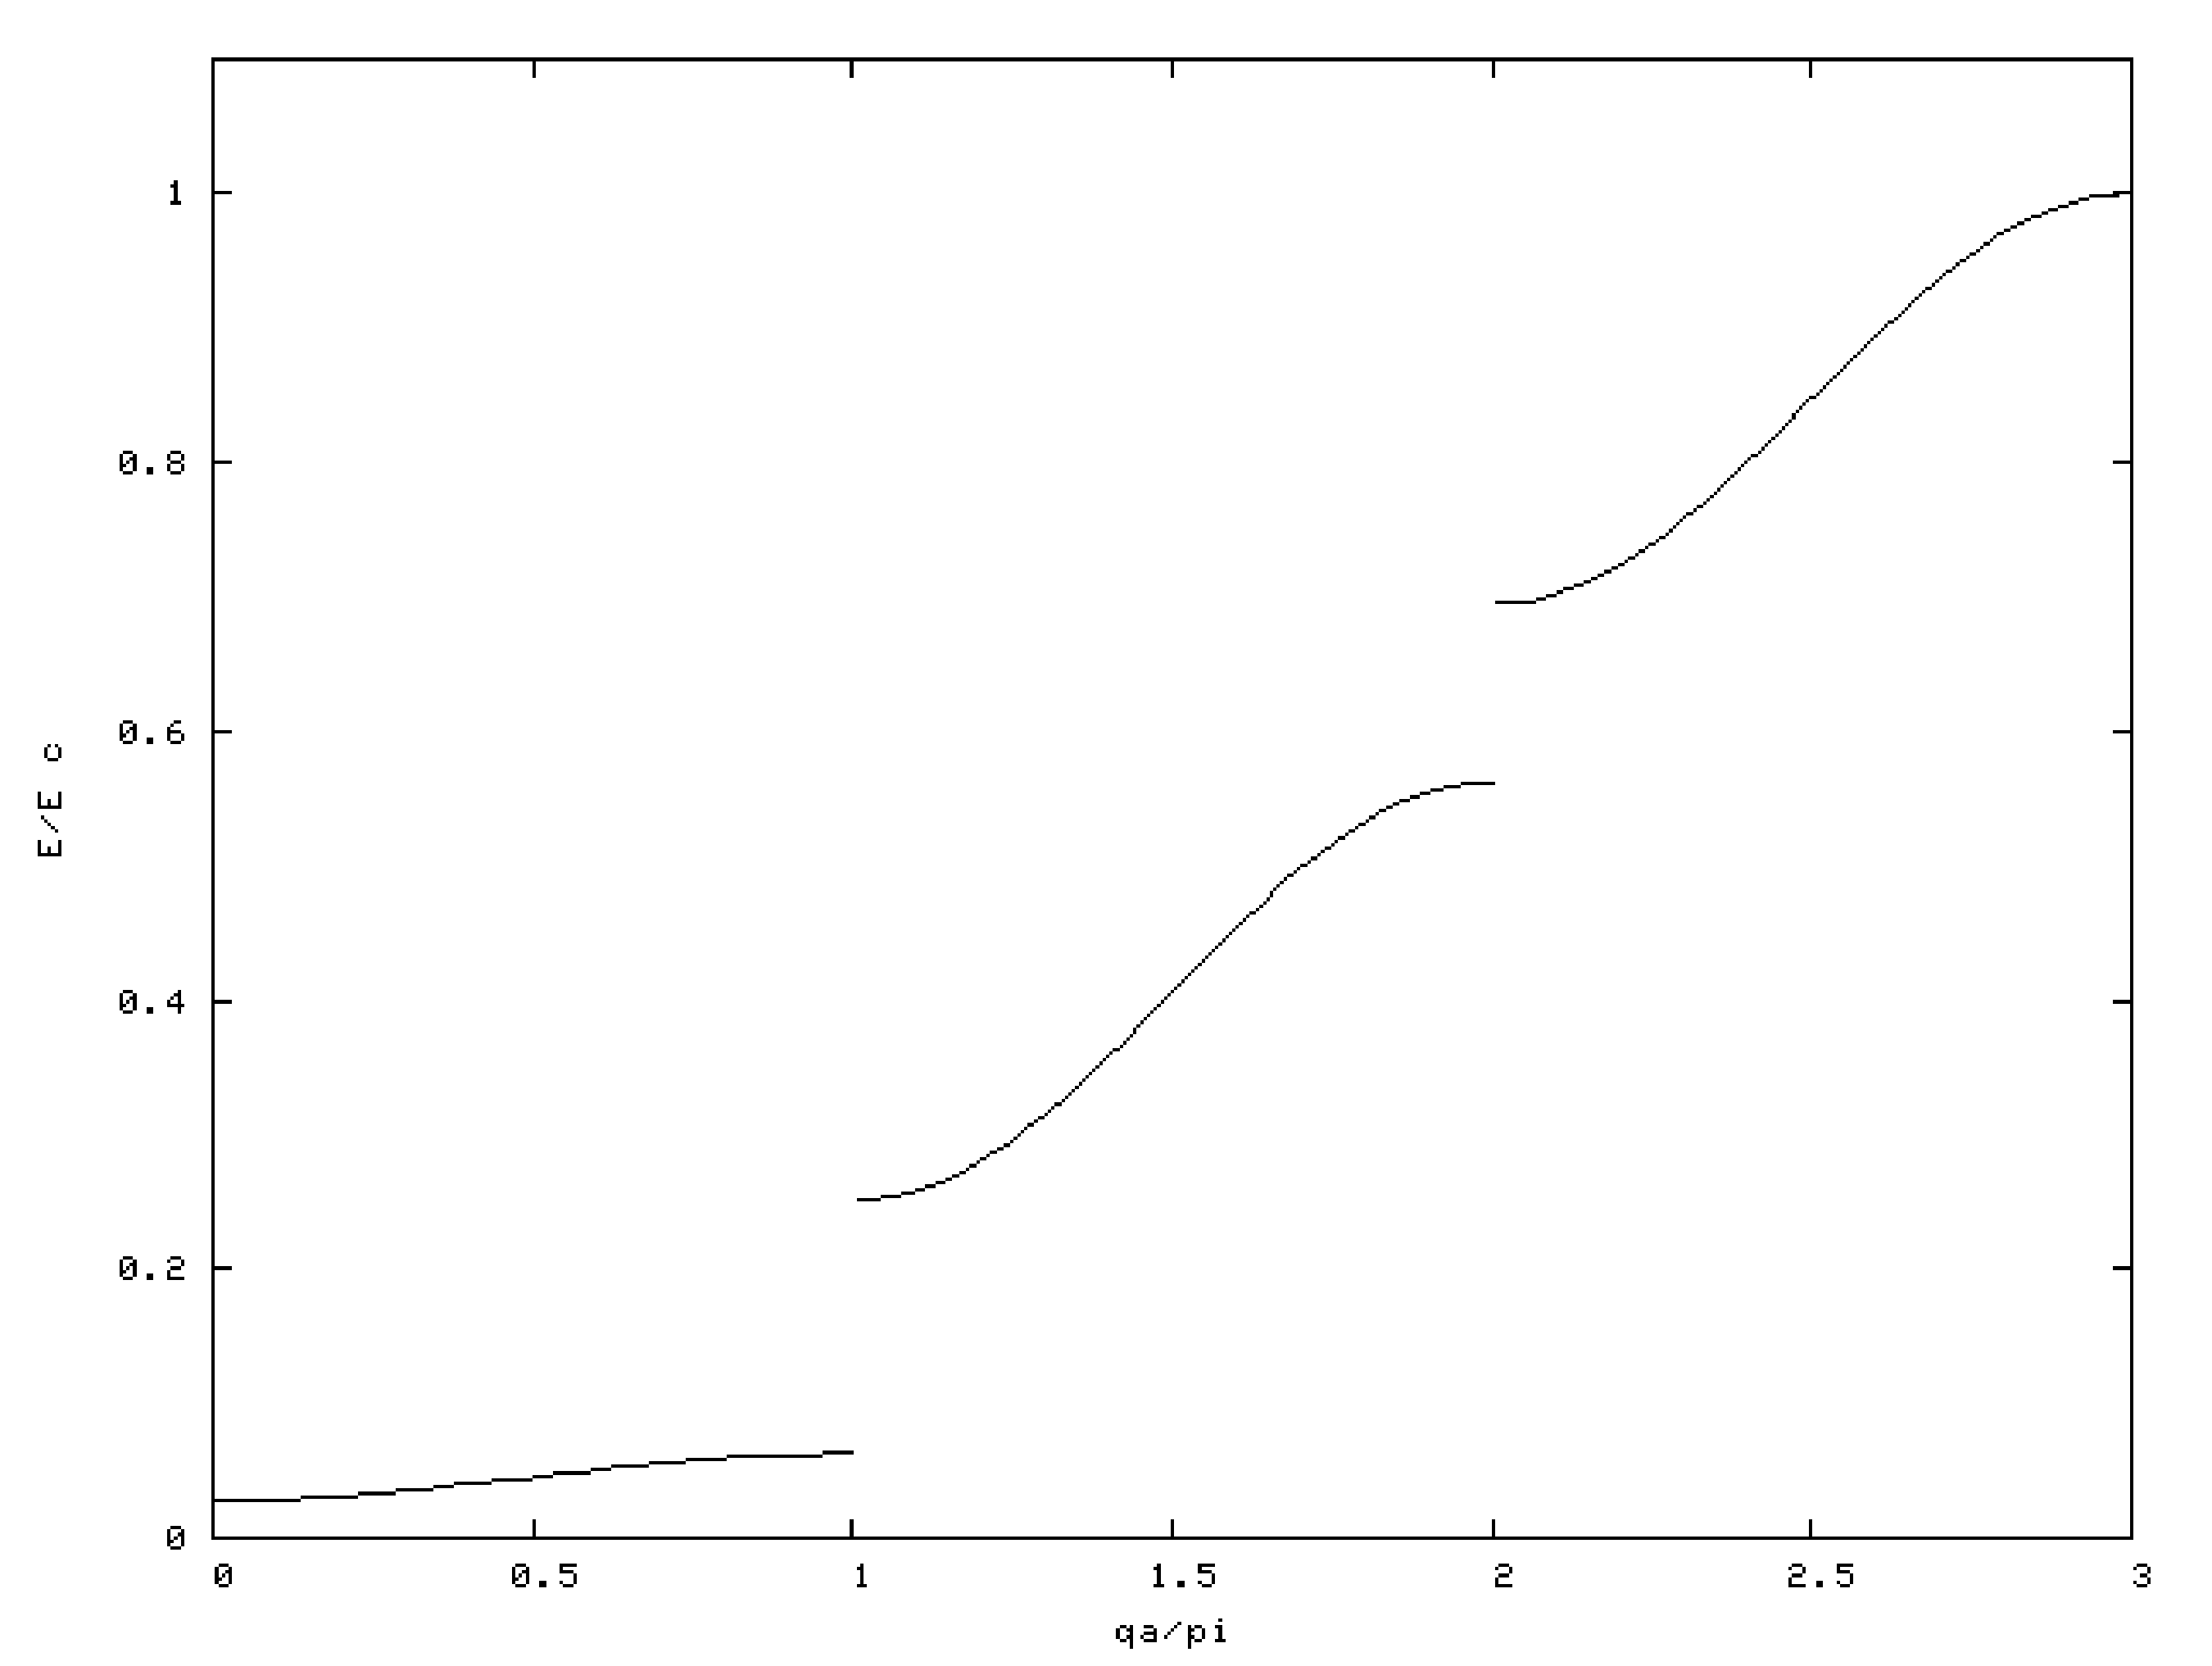
\includegraphics[width=110mm]{2003phy9-5.eps}
  \end{center}
\end{figure}

\end{enumerate}
\end{answer}
\end{document}
